%********************************************************************************************
%								COMANDOS ÚTILES PARA LATEX EN ESTE TP							
%
%	\ : espacio simple
%	\\ : nueva línea
%	\par : va a la línea de abajo y deja sangría
%	\vspace{##tamaño en pt##} o \vspace{\baselineskip} en general:
%								 para dejar un espacio vertical
%	\textbf{text} :text en negrita
%	\textit{text} :text en itálica
%
% GRAFICOS CENTRADOS:
%	\begin{center}
%		\includegraphics[width=\textwidth]{./img/##ruta imagen (no hace falta extension)##}
%	\end{center}
%		--> se pueden agregar atributos como scale por si se hace muy grande
%
% TABLAS CENTRADAS:
%	\begin{center}
%	\begin{tabular}{|c|c|}
%	\hline
%	\ \textbf{Programa} & \textbf{Ticks} \\
%	\hline
%		ASM & 675127609 \\
%	\hline
%	\end{tabular}
%	\end{center}
%
% ALGORITMOS (EN VARIOS LENGUAJES):
% \begin{lstlisting}
%	void sumoDiez(int &num)
%	{
%	    num += 10;
%	}
%	
%	int main()
%	{
% 	   int i;
%	    int numeroAProcesar = 20;
%	    for (i = 0; i < 50; i++)
%	    {
%	        sumoDiez(numeroAProcesar);	//Proceso el numero en cada ciclo
%	    } 
%	    return 0;
%	}
%	\end{lstlisting}
%
% para info sobre todo lo que tiene el package detallado:
% http://en.wikibooks.org/wiki/LaTeX/Source\_Code\_Listings
%
%********************************************************************************************

\documentclass[10pt,a4paper]{article}
\usepackage[utf8]{inputenc} % para poder usar tildes en archivos UTF-8
\usepackage[spanish]{babel} % para que comandos como \today den el resultado en castellano
\usepackage{a4wide} % márgenes un poco más anchos que lo usual
\usepackage[conEntregas]{caratula}
\usepackage{amssymb}
\usepackage{fancybox}
\usepackage[usenames,dvipsnames]{color}
\usepackage{hyperref}
\usepackage{listings}
\usepackage{xcolor}
\usepackage{amsmath}

\hypersetup{
    colorlinks,
    citecolor=black,
    filecolor=black,
    linkcolor=black,
    urlcolor=black
}

\lstdefinestyle{customc}{
  belowcaptionskip=1\baselineskip,
  breaklines=true,
  frame=L,
  xleftmargin=\parindent,
  language=C,
  showstringspaces=false,
  basicstyle=\footnotesize\ttfamily,
  keywordstyle=\bfseries\color{green!40!black},
  commentstyle=\itshape\color{purple!40!black},
  identifierstyle=\color{blue},
  stringstyle=\color{orange},
}

\lstset{escapechar=@,style=customc}

\begin{document}

\titulo{Trabajo Práctico 1}
\subtitulo{Análisis preliminar del sistema de software “TecnoTaxi”}

\fecha{\today}

\materia{Ingeniería del Software I}
\grupo{}

\integrante{Barbeito, Nicolás}{LLL/AA}{nicolasbarbeiton@gmail.com}
\integrante{Chapresto, Matías}{LLL/12}{matiaschapresto@gmail.com}
\integrante{Garassino, Agustín Javier}{394/12}{ajgarassino@gmail.com}
\integrante{Sarriés, Ana}{144/02}{anasarries@yahoo.com.ar}
\integrante{Vileriño, Silvio}{106/12}{svilerino@gmail.com}

\maketitle

\tableofcontents
\newpage

\section{Descripción general del sistema}
El objetivo del sistema es automatizar las solicitudes de taxis por parte de los pasajeros y la coordinación de los viajes con los taxistas. Para lograr esto se desarrollará una aplicación web, con la cual interactuarán tanto los clientes como los empleados de la empresa de RadioTaxi. Los pasajeros podrán comunicarse a través de internet para solicitar los viajes ya sea utilizando un dispositivo móvil o una computadora de escritorio. Tendrán la opción de elegir dentro de un listado de perfiles de choferes con información sobre: el modelo del auto, puntuación asignada según antiguos pasajeros, etc. A su vez los taxistas interactuarán con el sistema utilizando dispositivos móviles que serán proveídos por la empresa de RadioTaxi, ellos tendrán un listado de posibles viajes a realizar, pudiendo aceptar uno de ellos en cualquier momento. Además, con el fin de mejorar el servicio, información sobre la ubicación de los taxis será obtenida a través de un dispositivo de posicionamiento global GPS que se comunicará con el servidor web por medio de 3G.

\section{Interacción con el pasajero}
La interacción de la plataforma con el pasajero será, como se mencionó anteriormente, a través de internet. Para tener acceso al sistema este deberá primero crear un usuario, indicando un mail y contraseña. Esto permitirá posteriormente obtener información estadística de gran valor, además de permitir comunicarse con el pasajero en caso de que el viaje no pueda ser concretado por algún motivo. 

Un usuario puede solicitar un viaje a través de la aplicación web indicando el punto donde el taxi debe pasar a recogerlo, el destino y el horario. A esto la aplicación contestará con un listado de posibles taxistas elegidos convenientemente según las preferencias del usuario en base a información recopilada por el sistema, teniendo en cuenta también la ubicación actual de cada una de las unidades. El usuario puede proceder a seleccionar uno o varios de los taxistas, el sistema tendrá en cuenta la decisión del usuario pero el taxista al que se le asignará el viaje puede diferir.

Una vez determinado el taxista que se encargará del viaje el usuario será notificado. Finalmente el pasajero tendrá acceso a un menú de viajes pendientes en donde podrá visualizar la ubicación actual del taxi, además de tener la posibilidad de cancelar la solicitud. Una vez finalizado el viaje, el usuario puede puntuar al taxista positiva o negativamente. En caso de que el taxista cancele el viaje asignado, el usuario será notificado.

El pasajero podrá además utilizar la aplicación para reservar viajes periódicos seleccionando un taxista específico entre los disponibles. En caso de que por algún motivo el taxista no pueda concurrir uno de los días especificados el usuario será informado y otro taxista será ofrecido en su lugar.

En caso de no disponer de acceso a internet, el pasajero podrá llamar a un operador humano con acceso al sistema. No es necesario que el pasajero disponga de una cuenta en la aplicación, el operador realizará toda la interacción con el sistema. Sin embargo, dado el inconveniente de la p\'erdida de conex\'ion, se pierde parte de la funcionalidad del sistema, como el acceso al listado de taxistas. El pasajero que se comunique por tel\'efono s\'olo podr\'a solicitar un taxi cualquiera, cancelarlo y solicitar el tiempo de espera.

\section{Interacción con el taxista}
Los perfiles de los taxistas serán cargados manualmente en la aplicación. Tendrán un taxi asociado y una puntuación determinada por los usuarios a través de un sistema de votación. Estos serán informados cada vez que haya una solicitud de viaje que el sistema considere relevante al taxista en base a su ubicación actual. El taxista, disponiendo de toda la información asociada al viaje (destino, ubicación y hora) podrá aceptar o rechazar el viaje. En caso de aceptar una solicitud, será informado posteriormente si el viaje le es asigando. En caso de que el viaje le sea asignado, una vez que este se concrete deberá marcarlo como finalizado. En caso de no poder recoger a un pasajero por algún motivo, el taxista podrá en todo momento cancelar alguno de sus viajes pendientes, delegando la tarea de reasignar un nuevo taxista e informar al usuario al sistema.

\vspace{\baselineskip}
        \begin{center}
		    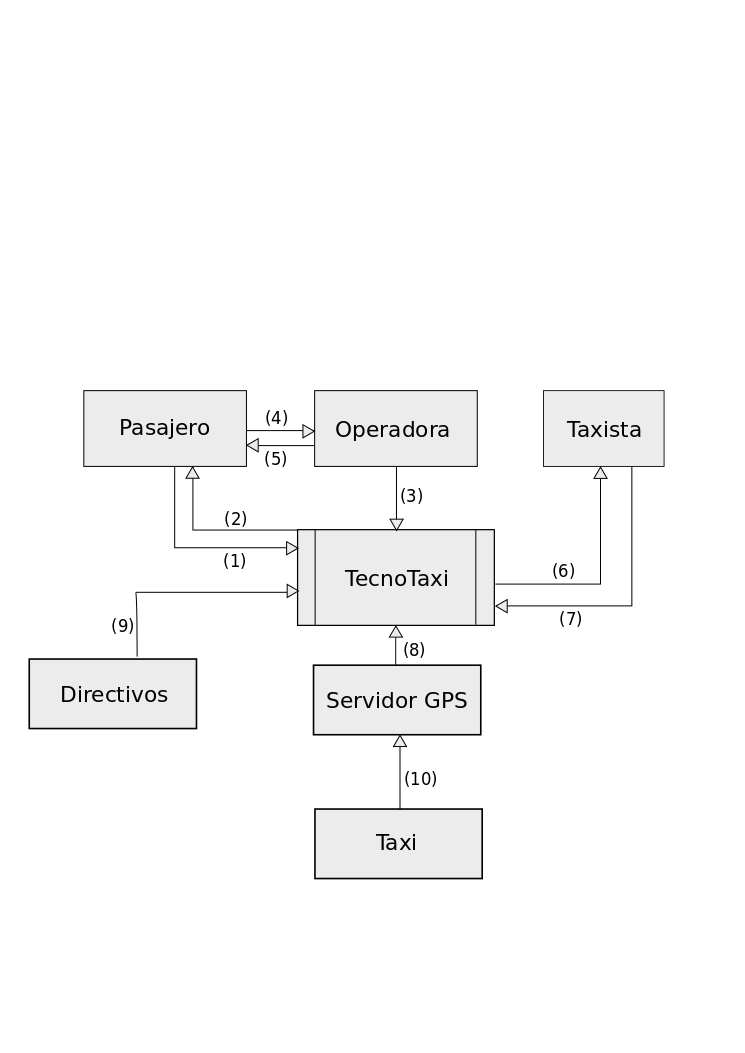
\includegraphics[scale=0.50]{contexto.png}
		    \\
		    \vspace{1pt}
		    \footnotesize\textit{Diagrama de contexto del sistema “TecnoTaxi”.}
	    \end{center}
    \vspace{\baselineskip}
\par 

\begin{enumerate}

    \item Pasajero $\Rightarrow$ TecnoTaxi
    \begin{itemize}
        \item Pasajero se registra en el sistema
        \item Pasajero solicita taxi a traves de internet
        \item Pasajero selecciona alguno (o ninguno) de los taxistas disponibles para confirmar el viaje
        \item Pasajero cancela viaje a traves de internet
        \item Pasajero otorga puntaje al taxista
        \item Pasajero solicita tiempo de espera del taxi a traves de internet
    \end{itemize}

    \item TecnoTaxi $\Rightarrow$ Pasajero
    \begin{itemize}
        \item Sistema ofrece listado de taxis disponibles para satisfacer solicitud de viaje
        \item Sistema informa el tiempo de espera del taxi 
        \item Sisema informa de cancelacion del viaje por parte del taxista
    \end{itemize}

    \item Operadora $\Rightarrow$ TecnoTaxi
    \begin{itemize}
        \item Operadora informa de un nuevo viaje solicitado
        \item Operadora informa de la cancelacion de un viaje
        \item Operadora solicita tiempo de espera del taxi
    \end{itemize}

    \item Pasajero $\Rightarrow$ Operadora
    \begin{itemize}
         \item Pasajero solicita taxi telef\'onicamente
         \item Pasajero cancela el pedido telef\'onicamente
         \item Pasajero solicita tiempo de espera del taxi telef\'onicamente
    \end{itemize}

    \item Operadora $\Rightarrow$ Pasajero
    \begin{itemize}
        \item Operadora informa el tiempo de espera del taxi
    \end{itemize}

    \item TecnoTaxi $\Rightarrow$ Taxista
    \begin{itemize}
        \item Sistema ofrece el viaje al taxista
        \item Sistema informa de cancelacion de viaje al taxista
    \end{itemize}

    \item Taxista $\Rightarrow$ TecnoTaxi
    \begin{itemize}
         \item Taxista acepta viaje ofrecido
         \item Taxista cancela viaje
         \item Taxista informa viaje completado
     \end{itemize}

    \item Servidor GPS $\Rightarrow$ TecnoTaxi
    \begin{itemize}
        \item GPS notifica cambio de posicion de un taxi
    \end{itemize}	

    \item Directivos $\Rightarrow$ TecnoTaxi
    \begin{itemize}
        \item Directivos consultan estadisticas del sistema.
    \end{itemize} 

    \item Taxi $\Rightarrow$ Servidor GPS
    \begin{itemize}
        \item Taxi cambia de posicion y es monitoreado por el Servidor GPS
    \end{itemize} 
\end{enumerate}

\end{document}
